%\documentclass[twoside,12pt]{book}
\documentclass[12pt]{book}
%\documentclass[oneside,12pt]{book}
\pagestyle{plain}

\usepackage[utf8x]{inputenc}
\usepackage[english, russian]{babel}
%\usepackage[dvips]{graphicx}
\usepackage[pdftex]{graphicx}
\usepackage{verse}

\usepackage[marginratio=3:2]{geometry}
\geometry{papersize={145mm, 205mm}}

% Убираем обязательные подписи к фотографиям (Рис.)
\usepackage{caption}

% Подключаем мантру правильных многоточий
% Взято отсюда http://kostyrka.ru/blog/archives/42

\usepackage{soulutf8,xspace} % у кого не UTF-8, те пишут просто soul
\xspaceaddexceptions{ < ) }
\sodef\so{}{.1em}{1em}{.3em plus.05em minus.05em}
\newcommand{\ldotst}{\so{...}\xspace}
\newcommand{\ldotsq}{\so{?\hbox{\hspace{-.212em}}..}\xspace}
\newcommand{\ldotse}{\so{!..}\xspace}

%\setcounter{secnumdepth}{0}

% Висячая пунктуация
%\usepackage[factor=2000]{microtype}
%\setlength{\oddsidemargin}{5mm}
%\setlength{\evensidemargin}{5mm}
% See more at: http://www.howtotex.com/tips-tricks/two-sided-latex-page-margins/#sthash.HA9tTo9O.dpuf

\begin{document}

%\frontmatter

% Нумерацию страниц начинаем с титульного листа:
\mainmatter

% Титульный лист
\begin{titlepage}
  \begin{center}

\vfill

{\huge Избранные стихотворения}

\vskip 5pt
{\large Егора Кузьмичева}

\vspace*{0.5cm}
\begin{figure}[htp]
  \begin{center}
	  \includegraphics[scale=0.6]{images/kuzmichev_oval.pdf}
%    \caption*{Егор Кузьмичев}
	  \caption*{1867--1933}
  \end{center}
\end{figure}
%{\center 1867--1933}
%{\LARGE Сборник стихотворений крестьянского поэта Волоколамского края Егора Кузьмича Кузьмичёва (1867--1933)}

\vfill
{\small
Москва

Издательство Кузьмичевых

2016
}
\end{center}
\end{titlepage}


%\pagenumbering{gobble}
\thispagestyle{empty}

\vbox to\textheight{

\hbox to\textwidth{%
\begin{tabular}[t]{@{}l@{ }l@{}}
%УДК&512.763+512.732\\% для математики находится по (неполной?) таблице УДК в~201
%ББК&22.147\\% находится по таблице ББК в~201
%&А61% находится по таблице авторских знаков в~201
\end{tabular}
\hss}

\vspace{3\baselineskip}

\hyphenation{МЦНМО}


{\settowidth{\leftskip}{А61\hskip1em}
\ifdim\overfullrule>0pt
\vbox to 0pt{\noindent\hskip-\leftskip\hskip-.5em \vrule height 6cm\vss}\fi
\noindent\textbf{Е. К. Кузьмичев}

%\noindent\hbox to 0pt{\hskip-\leftskip А61\hss}\hskip\parindent

Е. К. Кузьмичев

\vspace{2pt}
%{\small
%ISBN 978-5-94057-572-6}

\vskip.5\baselineskip

{\footnotesize
	Настала необходимость издать книгу поэзии крестьянского поэта Егора Кузьмича Кузьмичева (1867--1933), т.к. последнее крупное издание было в 1917 году. Пройдя сквозь век стихи приобрели ценность как документ эпохи. 
Его сугубо крестьянская лирика обращена к земле и считается продолжением крестьянской линии поэзии Сурикова, Никитина, Кольцова.
В поэзии крестьянского поэта сильна связь с народной песней. Стиль, мелодия, ритм – все звучит русским звуком.
Сохранилась книга 1917 года с рукописными авторскими правками. Составители издают обновленный текст стихов по авторским правкам.
\par
\vskip\baselineskip}

%\hbox to\textwidth{\hfil ББК 22.147}

}

\vfill

\hbox to\textwidth{%
\begin{tabular}[b]{@{}l}
%\textbf{ISBN 978-5-94057-572-6}
\end{tabular}
\hfill
\begin{tabular}[b]{@{}l@{ }l@{}}
%\copyright
%Е. К. Кузьмичев
%\copyright
%&МЦНМО, 200?
\end{tabular}}}
\clearpage


% Страница с описанием
% Мы ее исключили
% \include{description}


% Страница с фотографией автора
% \vspace*{2.5cm}
\begin{figure}[htp]
  \begin{center}
	  \includegraphics[scale=0.6]{kuzmichev_oval.pdf}
    \caption*{Егор Кузьмичев}
  \end{center}
\end{figure}





% Основная часть
%\mainmatter
%\setcounter{page}{3}
% Вступительная статья
%\include{intro}


% Стихотворения
% \chapter*{Стихотворения}
%% Текст сверяется с оригинальным изданием, вносятся очевидные грамматические исправления, при этом приводится пояснение (комментарий) и ссылка на академический источник-подтверждение. Оригинальными сохраняются также отступы. Используется окружение altverse. Для отступа в общем случае установлено 4 пробельных знака. 

\vspace*{0cm}
\poemtitle{Полет мысли}
\begin{verse}
\begin{altverse}
В живой любви тепла и света\\
Предела нет, и нет границ\\
Тоске и радости поэта, --- \\
Они на тысячах страниц\ldots\\
Слезами вписаны, пропеты, \\
При блеске розовых зарниц\ldots\\
% Правописание надо б
% http://www.evartist.narod.ru/text1/38.htm
Желаньям надо б утомиться,\\
Но жажда все еще живет,\\
И мысль летит, --- все дальше мчится\\
Под бурный шум, в круговорот,\\
К разгадке смелая стремится\\
% Нужна ли здесь запятая?
И --- неразгаданной умрет\ldots
\end{altverse}
\end{verse}
% Сверено с оригиналом. Исправлена пунктуация. Егор, Ольга 19.12.15 

\newpage
\vspace*{0cm}

\poemtitle{Дорогое детство}
\begin{verse}
\begin{altverse}
    Люблю я детство золотое,\\
В родной деревне прожитое,\\
    Люблю порою вспоминать:\\
Как в поле с матерью, бывало,\\
% По правилам пунктуации добавили запятую после вводного слова ``бывало''
% Ссылка http://new.gramota.ru/spravka/punctum?layout=item&id=58_76 
    Идешь в работе помогать,\\
% Вместо оригинального двоеточия после помогать поставлена запятая (по смыслу) 
Мы утро с радостью встречали,\\
Меня тогда не омрачали\\
    Заботы, бедность и тоска.\\
Я знал одно святое счастье, ---\\
    Любовь родимой глубока\ldots\\
Лишь взглянет мать: уж чуешь ласки,\\
Бежишь, горят, как угли, глазки,\\
    Огнем пылают сердце, грудь,\\
И знаешь, верно, у родимой, \\
% Перед словом верно добавлена запятая по правилам пунктуации
% http://new.gramota.ru/spravka/punctum?layout=item&id=58_267 
    Гостинец спрятан где-нибудь.\\
Иль ночью, в зимние метели,\\
В избушке теплой на постели\\
    Обнимет ласково рукой,\\
Опять в груди почуешь радость, \\
    Прильнешь к родимой головой\ldots\\
Давно то время миновало ---\\
Хранит земное покрывало\\
    В могиле тихой милый прах.\\
Уж стар и я, белеет иней\\
    В моих кудрявых волосах.\\
Но вспомнишь только лишь порою, ---\\
Воскреснет детство предо мною,\\
    И мир мне кажется другой\ldots\\
И снова матери желанной\\
Я вижу образ дорогой.
\end{altverse}
\end{verse}
% Сверено с оригиналом. Исправлена пунктуация. Егор, Ольга 19/12/15

\newpage
\vspace*{0cm}

\poemtitle{Палисадник}
\begin{verse}
\begin{altverse}
Мой любимый палисадник\\
    Светом солнечным залит,\\
Частокол его старинный\\
    Алым хмелем перевит;\\
Распустилася малина,\\
    Вишни, яблони цветут,\\
И смородина меж ними\\
    Разметалась там и тут;\\
Пчелы вьются над кустами,\\
    Собирая сладкий мед,\\
И пестреет над лужайкой\\
    %Мотыльковый хоровод,\\
	Мотыльковый хоровод.\\
А под вербой, ближе к тыну, ---\\
    Заповедная скамья,\\
Где в тени, в часы досуга,\\
    Отдыхает вся семья\ldots\\
Здесь надежды воскресают\\
    И безмолвствует вражда,\\
Забываются обиды,\\
    Гнет, и горе, и нужда.
\end{altverse}
\end{verse}

\newpage
\vspace*{0cm}


% Сверено с оригиналом. Егор, Ольга 19/12/15 


\poemtitle{В погоне за юностью}
\begin{verse}
О, юность, юность, погоди\ldotse\\
Моя звезда не закатилась,\\
Она позднее засветилась, ---\\
% Строка поправлена по книге с авторскими правками 
Надежда-радость впереди\ldotse\\
% Строка поправлена по книге с авторскими правками 
Еще цветы не отцвели,\\
Мороз не выжал аромата,\\
И красотою жизнь богата, ---\\
Лишь только жажду утоли\ldotst\\
Умерь свой бег, и дай скорей\\
Хоть миг желанного привета\ldotst\\
% По правке 
И поспешим с тобою к свету\\
% По правке 
Весенней молнии быстрей\ldotst
\end{verse}

\newpage
\vspace*{0cm}


\poemtitle{Мужик}
\begin{verse}
\indentpattern{101010101010}
\begin{patverse}
\vinВечно суровую, рабскую долю\\
Тянет забитый, голодный мужик;\\
С детства узнал он нужду и неволю,\\
С детства к терпенью покорно привык.\\
Вечно идет он тяжелой дорогой,\\
Потом он землю чужую поит\ldotst\\
Труженик честный, обиды он много\\
С болью на сердце на время таит\ldotst\\
Грудью стоит он за землю родную, \\
Первая жертва в кровавом бою.\\
Он ли не выстрадал долю иную,\\
Право на землю родную свою\ldotsq
\end{patverse}
\end{verse}

\newpage
\vspace*{2cm}
 
\poemtitle{Размышление}
\begin{verse}
\begin{altverse}
К чему о правде рассужденья,\\ 
%   Было:
%   Пророком что-ли хочешь быть\ldotse\\
    Пророком что ли хочешь быть\ldotse\\
Оставь напрасные волненья, ---\\
    Спокойно лучше в мире жить.\\!

Не трогай нервы, равнодушно\\
    Смотри, где льется пот и кровь\ldotst\\
Тебе ли быть великодушным?!\\
    Их ждет борьба, а не любовь.\\!

А ты? Ты жалкий, ты ничтожный,\\
    Тебе ль страданье превозмочь?!\\
Тебя пугает шум тревожный,\\
    Гони мечты, гони их прочь!\\!
\end{altverse}
\vin\ldots\ldots\ldots\ldots\ldots\ldots\ldots\ldots\ldots\ldots\\!
\begin{altverse}
Нет, лжешь позорно, подлость злая,\\
    И тем волнуешь ум сильней,\\
В неистовстве изнемогая,\\
    Я с правдой выступлю смелей.\\!

Презренье брошу я кумиру,\\
    И с ним упитанным жрецам;\\
Иль разобью во гневе лиру,\\
    И, как червяк, --- погибну сам.
\end{altverse}
\end{verse}

\newpage
\vspace*{0cm}


\poemtitle{Березы}
\begin{verse}
\begin{altverse}
    Люблю я белые березы,\\
Как близких, ласковых друзей\ldotst\\
    На них росинки, словно слезы,\\
Чаруют прелестью своей\ldotst\\
    %Дрожат листы и нежный шепот\\
	Дрожат листы, и нежный шепот\\
О тайне вещей говорит:\\
    <<Оставь, безумец, дерзкий ропот,\\
Твоя звезда еще горит;\\
    Еще огни не угасали\\
Там, где витает мысль твоя,\\
    От преждевременной печали\\
Уйди в небесные края\ldotst\\
    И окрыленною мечтою\\
Простор далекий облети,\\
    Отдайся грезам и покою\\
В волшебном, облачном пути.\\
% Сейчас делаем ветку с авторской пунктуацией, затем сделаем ветку под корректуру. Корректура нужна, потому как есть спорные пунктуационные моменты и нужен профессиональный корректор.
    И, отдохнув душою, снова\\
Вернись к друзьям с запасом сил,\\
    С любовью пламенного слова\\
Скажи, что в тайне пережил;\\
    Утешь их вечной чудной сказкой\\
Лазурных солнечных высот,\\
Как был ты встречен с теплой лаской\\
%Было (в оригинале)
%Среди божественных красот>>..
%Стало (исправил) - Г.К.
Среди божественных красот...>>
\end{altverse}
\end{verse}


\newpage
\vspace*{0cm}


% Как думаешь, как сделать поиск в новой книге?
% Может, нужен индекс? - Список стихов по алфавиту.
% - Возможно ли установить даты написания стихов и отсортировать их по дате написания или по году написания? 


% Старое название - ``Весна проснулась'' - c 182
\poemtitle{Веснянка}
\begin{verse}
\begin{altverse}
Проснулась жизнь, любовью дышит,\\
    По жилам кровь быстрей бежит\ldotst\\
Зеленый лес листвой колышет,\\
    Под пенье птиц вокруг шумит\ldotst\\
Стада пасутся\ldotst Вниз долины\\
    Ручей извилистый гремит,\\
Таясь в тени густой калины,\\
% Вот здесь вопрос, что поставить вместо этого авторского выбора пунктуации ..,
%    Веснянка юная стоит..,\\
     Веснянка юная стоит\ldotst\\
Прекрасный взгляд ее, лукавый,\\
    Скользит с улыбкой по ручью\ldotst\\
% Здесь дефис стоит после запятой. Ставить его или нет? А вдруг нет? Место мало, вот и поставил. Запятая с тире вполне себе употребляется в языке. Другой вопрос, уместно ли это в данном случае? - Это к редактору книги. Кто редактор книги. Не я. А кто? Это надо найти редактора и корректора. 
%Вдали, --- рыбак взошел на лавы,\\
Вдали --- рыбак взошел на лавы,\\
    И чинит легкую ладью\ldotst\\
На миг мелькнула грудью белой\\
    Краса веснянки в камышах,\\
%И, поплыла как лебедь, смело,\\
И поплыла, как лебедь, смело,\\
    Играя брызгами в волнах;\\
И лишь пестреет золотистый\\
    Наряд красавицы в лугах\ldotst\\
Склонился ландыш серебристый\\
    К фиалке бархатной в кустах\ldotst\\
Шепча любовно лепестками,\\
    Фиалка ловит страстный взгляд\ldotst\\
Сплелися нежно стебельками,\\
    И льют душистый аромат\ldotst
\end{altverse}
\end{verse}

\newpage
\vspace*{0cm}


\poemtitle{Зима}
\begin{verse}
\indentpattern{01010101010101010101}
\begin{patverse}
Все вокруг в природе\\
Сном могильным спит,\\
В стройном хороводе\\
Лес седой стоит,\\
На деревьях иней\\
Серебром блестит,\\
А вдали свод синий\\
Над землей висит\ldotst\\
И река под снегом\\
Замерла в тиши;\\
Лишь метель, набегом,\\
Прошумит в глуши,\\
Засвистит в прибрежных\\
Камышах сухих,\\
Злобно пылью снежной\\
Обдавая их.\\
И растут все выше\\
Берега кругом, --- \\
Расписные крыши\\
И за домом дом\ldotst
\end{patverse}
\end{verse}

\newpage
\vspace*{0cm}


% Страница 54
\poemtitle{Заколдованный лес}
\begin{verse}
\indentpattern{010101010101}
\begin{patverse}
Лес поредел, валятся листья,\\
Деревья хмурые стоят, ---\\
И жутко темными ветвями\\
В сыром тумане шелестят\ldotst\\
Семья лишайников желтеет,\\
Зубцы раскинув по земле;\\
Осины прелой пряный запах\\
Висит в дрожащей полумгле.\\
Заснуло все\ldotst Лишь дятел где-то\\
Порою, стукнет по сосне,\\
И снова тишь\ldotst И тяжко дышит\\
Лес заколдованный во сне\ldotst
\end{patverse}
\end{verse}

\newpage
\vspace*{0cm}


% 104
\poemtitle{Не ходи\ldotst}
\begin{verse}
\begin{altverse}
Не ходи, нужда, за мною,\\
    По моим следам ---\\
Снег растает, я весною\\
    Все тебе отдам:\\
Закопченную лачугу\\
    И чердак пустой,\\
Где зимою слушал вьюгу\\
    За трубой худой.\\
Все возьми --- мои онучи,\\
    Рваный мой озям\ldotst\\
Я пойду туда, за кручи,\\
    К солнцу, к небесам\ldotst\\
Где свободно будет можно\\
    Воздухом дышать,\\
Где не надо жизнью ложной\\
    Душу омрачать\ldotst\\
\end{altverse}
\end{verse}

\newpage
\vspace*{0cm}

% P. 132
\poemtitle{Возвращение}
\begin{verse}
\begin{altverse}
Душа наполнилась мольбою\\
    И вера вспыхнула в груди,\\
Как будто реет предо мною\\
    Святое счастье впереди.\\!

Опять я вижу парк старинный\\
    И слышу лип кудрявых шум,\\
Листвы зеленой шепот дивный\\
    Волнует мой усталый ум.\\!

Гляжу я в даль, где речка вьется\\
    Между лощин по скату гор,\\
И чую --- сердце жадно рвется\\
    Туда --- на волю, на простор.
\end{altverse}
\end{verse}

\newpage
\vspace*{0cm}


% Page 109
\poemtitle{Нет, не хочу\ldotst}
\begin{verse}
\begin{altverse}
%Надо-ль коварной судьбе покорятся\ldotsq\\
Надо ль коварной судьбе покоряться\ldotsq\\
    Правда ль, что рабство дано мне в удел?\\
Нет\ldotse Не хочу больше бури бояться,\\
    %Вырву тот страх, чем я с детства болел. ---\\!
	Вырву тот страх, чем я с детства болел.\\!
Высушил грудь, и усталые руки\ldotst\\
    Жизнь не хочу я в цепях потерять,\\
Вынес я много обмана и муки, ---\\
    Ложь вековую пора мне понять\ldotst\\!

Сбросить пора мне оковы насилья,\\
    Слепо мириться теперь не хочу,\\
Я разверну угнетенные крылья,\\
    Вольною птицею ввысь полечу\ldotst
\end{altverse}
\end{verse}


\newpage
\vspace*{0cm}

% P 191
\poemtitle{Другу}
\begin{verse}
\begin{altverse}
Не вини меня, друг милый,\\
    Что пою про скорбь да муки\ldotst\\
Про того мой стих унылый,\\
    У кого в мозолях руки\ldotst\\!

Стал бы петь, как плещет море,\\
    Ходят волны голубые,\\
Да повсюду стонет горе,\\
    Гибнут близкие, родные\ldotst\\!

%О лесах бы спел дремучих\\
О лесах бы спел дремучих,\\
    О красе лугов душистых,\\
Да вокруг так много жгучих\\
    Горьких слез, невинных, чистых\ldotst\\!

Спел бы я про вечер сонный,\\
    О метелях в зимний холод,\\
Сердце рвет неугомонный,\\
    Словно зверь, народный голод.\\!

Я бы спел про взгляд прекрасный,\\
    Чем подруга подарила,\\
Да сдавил кошмар ужасный,\\
    Грудь тоска мне защемила\ldotst
\end{altverse}
\end{verse}

\newpage
\vspace*{0cm}

% Page 156  
\poemtitle{Поздней осенью в лесу}
\begin{verse}
% Порядок строк поменян в соответствии с авторской правкой
Листы опали, даль бледнеет,\\
И заковало речку льдом,\\
И солнце красное не греет,\\
В лесу угрюмом и пустом;\\
\begingroup
\leftskip1em
\rightskip\leftskip
Не веет он волшебной сказкой\\
На думы грустные мои,\\
Туманя взор седою краской\\
Осин и тлеющей хвои.\\
\endgroup
Угасла жизнь, лишь мышь листвою\\
Шурша, нарушит тихий сон,\\
Да скрипнет дерево порою,\\
И эхо даст протяжный стон.
\end{verse}

\newpage
\vspace*{0cm}

%162
\poemtitle{Береза}
\begin{verse}
\begin{altverse}
Ты березынька,\\
    Ты кудрявая,\\
Одинокая,\\
    Сиротой стоишь;\\
А вокруг тебя,\\
    В речке плавая,\\
Шепчет ласково\\
    Молодой камыш:\\
<<Где укроюсь я\\
    В непогожий день,\\
Если бурная\\
    Речка вспенится\ldotse\\
Кто возьмет меня\\
    Под густую тень,\\
Когда солнышком\\
    Буря сменится?>>\\
Вдруг березынька\\
    Белоствольная\\
%Расшумелася\\
Расшумелася,\\
    Раскачалася:\\
<<Ах, когда бы мне\\
    Воля вольная, ---\\
Всю бы жизнь с тобой\\
    Я шепталася.\\
Распустила бы\\
    Сень ветвистую, ---\\
Пусть над реченькой\\
    Дремлет гладь и тишь!\\
Целовала б я\\
    Золотистую\\
Красоту твою,\\
    Молодой камыш!..>>
\end{altverse}
\end{verse}

\newpage
\vspace*{0cm}

%136
\poemtitle{Люблю}
\begin{verse}
\begin{altverse}
    Люблю я истину,\\
Люблю в добро святую веру,\\
    И не поддамся я\\
В обман ханже и лицемеру.\\!

    Да будет крест на век\\
Моей звездою путеводной!\\
    С ним, не страшась, пойду\\
Глухой тропой, в степи бесплодной\ldotst\\!

    В душе своей создам\\
Я светлый рай --- жилище Бога,\\
    И будет счастьем мне\\
В лучах любви к добру дорога\ldotst
\end{altverse}
\end{verse}

\newpage
\vspace*{0cm}

%211
\poemtitle{В дороге}
\begin{verse}
\indentpattern{01202020202020202020}
\begin{patverse}
Холод\ldotst Пасмурно в лесу\ldotst\\
   Лист увядший на дороге\\
      %Прилипает к колесу\\
	  Прилипает к колесу,\\
И гремят по корням дроги\ldotst\\
      Через мост с дровами воз\\
Еле тянет лошаденка,\\
      Как и прежде, так же бос,\\
Мужичок в худой шубенке\\
      Тихо за возом идет,\\
Бледный, с впалыми щеками,\\
      На лице все тот-же гнет,\\
Не смываемый веками\ldotst\\
      С ним и голод, с ним и страх\\
Идут рядом неразлучно\ldotst\\
      Яд у бедного в устах,\\
А на сердце скучно, скучно\ldotst\\
      Темнота\ldotst и, нем язык\\
За себя сказать не может,\\
      Мужичок терпеть привык,\\
А судьба-змея все гложет.
\end{patverse}
\end{verse}

\newpage
\vspace*{0cm}


%%% Откуда это??????? 
\poemtitle[<<Не унывай, душа моя...>>]{***}
\begin{verse}
\begin{altverse}
Не унывай, душа моя,\\
Что темен путь, трудна дорога!\\
    Стремись к добру, огнем горя…\\
Любить кто хочет свет и Бога –\\
Пред тем во тьме горит заря.
\end{altverse}
\end{verse}

\newpage
\vspace*{0cm}


%173
\poemtitle{Служи добру}
\begin{verse}
Служи добру, люби природу,\\
И в ней учись искать свободу,\\
Отбрось позорный, рабский страх, ---\\
Ведь ты родился не в цепях\ldotst\\!

Взгляни вокруг, --- примеров много:\\
Идут тернистою дорогой\\
Другие люди с юных лет;\\
У них в душе один завет ---\\!

Добыть себе иную долю,\\
%Иль гибнуть всем в борьбе за волю\\
Иль гибнуть всем в борьбе за волю,\\
И память тяжких черных дней\\
Украсить жертвою своей\ldotst
\end{verse}

\newpage
\vspace*{0cm}


%194
\poemtitle{Святая ночь в деревне}
\begin{verse}
\begin{altverse}
<<Христос воскрес!>> --- вещают миру\\
    %Святая ночь и, небеса,\\
	Святая ночь и небеса,\\
Вокруг, в проталинах пестрея,\\
    Поля, и темные леса\ldotst\\
<<Воскрес Христос!>> --- порвав оковы,\\
    Лепечет вольная река,\\
И в темь глубокую --- свободу\\
    Несет с собой издалека\ldotst\\
Бодрит весенний воздух свежий,\\
    Дрожит пасхальный перезвон\ldotst\\
Толпами шумными крестьяне\\
    Во храм идут со всех сторон;\\
Спешат услышать голос правды,\\
    Что мир настал, --- Христос воскрес\ldotst\\
Любовь повеяла на землю ---\\
    Весной душистою с небес\ldotst\\
\end{altverse}
\end{verse}


\newpage
\vspace*{0cm}


%262
\poemtitle{Любовь}
\begin{verse}
\begin{altverse}
Любовь!.. Как жгучи эти звуки!\\
    От них огонь горит в груди,\\
И утихают злые муки,\\
    И светит счастье впереди...\\
Любовь, как солнышко в лазури\\
    По небу синему плывет,\\
Порой среди страстей и бури\\
    С улыбкой тихо подойдет...\\
Обнимет крепко, безмятежно,\\
    Истомой сладкой обожжет...\\
И в поцелуе долгом, нежном,\\
    Нектаром сердце обольет...\\
\end{altverse}
\end{verse}

\newpage
\vspace*{0cm}


%275
\poemtitle{Под голубым небом}
\begin{verse}
\begin{altverse}
Тихо шепчется фиалка\\
    С василечком молодым,\\
Он сулит любовь и ласку\\
    Ей под небом голубым:\\
<<Зацветем под жгучим солнцем\\
    Краше прежнего, мой друг,\\
Пусть над нами раздаются\\
    Песни вольные вокруг>>...\\
А лучи тепла и света\\
    Льются, льются с высоты,\\
Опьяняют и ласкают\\
    Дивным блеском красоты...\\
Распылалася фиалка\\
    Страстью нежной к васильку,\\
И склонилась с поцелуем\\
    К молодому стебельку...\\
\end{altverse}
\end{verse}


\newpage
\vspace*{0cm}


%209
\poemtitle{Ты не со мной}
\begin{verse}
\begin{altverse}
Мой друг, зачем ты омрачила\\
     Безумной ревностью любовь\ldotsq\\
Во мне огонь, и страсти сила\\
     Лишь для тебя волнует кровь\ldotst\\!

Ложусь в постель, твой образ снится,\\
     До утра реет надо мной,\\
И грудь моя в тоске томится, ---\\
     Зачем я, друг мой, не с тобой\ldotst\\!

Пойду ль вечернею порою\\
      За речку слушать соловья,\\
Туман ложится полосою,\\
      И в нем твой призрак вижу я\ldotst\\!

Спешу дрожащими руками,\\
    Тебя обнять, поцеловать,\\
Но призрак тает пред глазами,\\
      Порыв заставив проклинать\ldotst\\!

Один с глубокою  тоскою,\\
     Застыв в безмолвной тишине,\\
Стою в раздумье над рекою,\\
     Мечтою полон о тебе\ldotst\\!

Вокруг глухая ночь темнеет,\\
       Вдали чуть слышен соловей,\\
Больное сердце холодеет\\
        В груди истерзанной моей\ldotst\\!

Стою и --- грусть в душе лелею\\
     К тебе, мой ангел дорогой,\\
И об одном лишь я жалею,\\
  Что нет тебя, мой друг, со мной\ldotst
\end{altverse}
\end{verse}

\newpage
\vspace*{0cm}


%251
\poemtitle{Не забуду}
\begin{verse}
\indentpattern{10101010101010101010101010101010}
\begin{altverse}
    Ты мне сказала: <<Позабудь!>>\\
Но я, мой ангел, не забуду\ldotst\\
     При первой встрече где-нибудь\\
В твоих объятьях снова буду\ldotst\\
     %А --- нет, то в грезах золотых\\
	  А нет --- то в грезах золотых\\
Тебя увижу ночью темной,\\
      О счастье дней пережитых\\
Мечтать я буду с грустью томной.\\
     С тобою жизнь моя цвела\ldotst\\
Я помню ветхое оконце,\\
     Где занавесочка была\\
Тобой повешена от солнца\ldotst\\
     Как были ночи хороши,\\
Когда туда ты провожала.\\
     И в заколдованной тиши\\
Обнявши крепко, целовала\ldotse\\
     Поутру, раннею зарей,\\
Будить ходила на рассвете\ldotst\\
     Ах\ldotst Сколько радости порой\\
% Нужен ли тут вопросительный знак? Или восклицательный?
Я видел в ласковом привете\ldotse\\
На грудь с душевной простотой\\
Спешишь ко мне ты наклониться...\\
Даешь, любуясь красотой,\\
Желаньем сладостным упиться...\\
Прошла пора весны моей,\\
С тоскою осень наступает,\\
А память летних теплых дней\\
В душе моей не умирает...\\
Могу ли солнца луч забыть,\\
Который в холод сердце греет,\\
И милый призрак разлюбить,\\
Что нежно так душа лелеет\ldotsq
\end{altverse}
\end{verse}

\newpage
\vspace*{0cm}

%94
\poemtitle{Расписной положок}
\begin{verse}
\begin{altverse}
%Ах, придется-ль когда\\
Ах, придется ль когда\\
   Мне тебя приласкать\ldotsq\\
Мне к другому теперь\\
   Тяжело привыкать...\\!

Помнишь, --- как горячо\\
    В положке обняла\ldotsq\\
С тех пор душу тебе,\\
    Милый друг, отдала\ldotst\\!

Ни запить, ни заесть\\
    Поцелуи твои, ---\\
Глубоко у меня\\
    Они в сердце легли\ldotst\\!

Примирилась с другим,\\
    Покорилась судьбе,\\
Но желанья мои\\
    Улетают к тебе, ---\\!

В расписной положок,\\
    На кроватку твою,\\
% нужна ли запятая? 
% Где ты, в сладостном сне\\ 
Где ты в сладостном сне\\
    Нежишь душу мою...
\end{altverse}
\end{verse}

\newpage
\vspace*{0cm}

% 222
\poemtitle{Она ждала}
\begin{verse}
\begin{altverse}
Она ждала и в даль глядела\\
    За синь туманную лесов,\\
И многое сказать хотела,\\
% В оригинале:
% Но, сердце мучилось без слов
    Но сердце мучилось без слов\ldotst\\
Она ждала, --- и без надежды\\
    Минуту счастья увидать ---\\
Ей заколдованные вежды\\
    Нельзя свободно поднимать\ldotst\\
% В оригинале:
% Но, в тайниках души несмелой
Но в тайниках души несмелой\\
    Горела пламенная страсть ---\\
Любви запретной, онемелой\\
    Бесследно миг не мог пропасть\ldotst\\
Она ждала\ldotst Порой мятежной\\
    Готова друга догонять, ---\\
% В отчаяньи --- ?
В отчаянье --- с улыбкой нежной\\
    Скрывая страх, его обнять\ldotst\\
%Она ждала --- смотря в оконце ---\\
Она ждала, смотря в оконце,\\
    Без сна, по целым по ночам,\\
Ждала с зарей, --- при свете солнца,\\
    Доверясь ласковым лучам.\\
Она ждала. Но --- ведьма злая\\
    К ней путь-дорогу замела,\\
%И вместо радостей, --- немая\\
И, вместо радостей, немая\\
    Тоска на сердце залегла.
\end{altverse}
\end{verse}

\newpage
\vspace*{0cm}


\poemtitle{Листок}
\begin{verse}
\begin{altverse}
Как много вдруг напомнил мне\\
     Листок бумаги белой!\\
Здесь были вписаны слова \\
     Ее рукой несмелой\ldotst\\
Здесь скрыта нежная любовь\\
     Ее глубокой страсти, ---\\
Водила милая пером\\
     Скрываясь от напасти\ldotst\\
% В оригинале Что-б
Чтоб зависть злобная людей\\
     Любви не омрачила, ---\\
Горячей искренной слезой\\
     Листочек омочила\ldotst\\
И, как молчания печать,\\
     К листку уста прижала\ldotst\\
С печалью томною в глазах ---\\
     Прощаясь, уезжала\ldotst\\
И тайну чуткую теперь\\
     Хранит листочек белый\\
Следы, что к сердцу провела\\
     Она рукой несмелой\ldotst\\
\end{altverse}
\end{verse}

\newpage
\vspace*{0cm}


% 83
\poemtitle[<<Ниже, ниже наклоняйтесь>>]{***}
\begin{verse}
\begin{altverse}
Ниже, ниже наклоняйтесь\\
Серебристые березы,\\
Чтобы люди не видали\\
На моих ресницах слезы;\\
Чтобы с милым про свиданье\\
Я одна бы только знала\ldotst\\
%Утони же, глубже, тайна,\\
Утони же глубже тайна,\\
Там, где вишня расцветала,\\
Где цветы ее под нами\\
Белым снегом рассыпались,\\
И листы зеленой груши\\
Тихо, ласково шептались.\\
Зарастай моя дорожка,\\
Где я с милым проходила,\\
Поломалася малина,\\
Что весною посадила.\\
Оклевали птицы вишню\\
И черемуху густую\ldotst\\
Грустно мне глядеть под вязы\\
На скамеечку пустую\ldotse\\
Солнце спряталось за тучку,\\
Мглой мой садик одевает,\\
И холодный, резкий ветер\\
Листья желтые срывает\ldotst\\
\end{altverse}
\end{verse}


\newpage
\vspace*{0cm}


%227
\poemtitle{Замужем}
\begin{verse}
\begin{altverse}
Радость, счастие --- далеко,\\
    Больше их не увидать\ldotst\\
Так вздыхаючи глубоко\\
    Буду вечно вспоминать\\
О девичей вольной доле,\\
    Как у матушки родной\\
Я росла в любви и холе,\\
    Земляничкою лесной\ldotst\\
% Здесь в коце либо точка, либо двоеточие... в двух книгах
Я в засеночках белела:\\
    В новом браном пологу,\\
И на солнышке алела\\
    Я, резвяся на лугу\ldotst\\
Русу косыньку чесала\\
    Нежно матушка моя,\\
На задворках запевала\\
    В хороводах первой --- я\ldotst\\
Добры-молодцы гналися\\
    За моею красотой\ldotst\\
Но, те годы пронеслися\\
%%%% Тире так в оригинале
%    --- Безвозратною мечтой\ldotst\\
    Безвозратною мечтой\ldotst\\
Непробудно спит в могиле\\
%    Мать родимая моя.\\
    Мать родимая моя,\\
И досталось не по силе\\
    Мне коварная семья:\\
Злою ревностью изводит\\
    Муж, как старый домовой\ldotst\\
А свекровь, косырясь, ходит,\\
    Смотрит тучей грозовой\ldotst\\
За красу мою золовки\\
    Ненавидят и корят,\\
Провинятся в чем плутовки ---\\
    На меня наговорят\ldotst\\
%Деверья, --- те защипают\ldotst\\
Деверья --- те защипают\ldotst\\
    И не смею оттолкнуть.\\
Свекор с бабушкой пытают,\\
    Целясь метко упрекнуть\ldotst\\
Не с кем горюшко размыкать,\\
    Мне без матушки родной\ldotst\\
%%%% В оригинале через дефис
%Как-бы хуже не накликать\\
Как бы хуже не накликать\\
    В горьких думушках одной!\\
\end{altverse}
\end{verse}

\newpage
\vspace*{0cm}


%9
\poemtitle{Не мне}
\begin{verse}
\begin{altverse}
Что --- <<море лишь одно свободно,\\
%А люди, --- жалкие рабы,>> ---\\
А люди --- жалкие рабы,>> ---\\
Не мне, не мне она сказала\\
%В пылу желаний и мольбы\\!
В пылу желаний и мольбы!\\!
%В оригинале стоит !.
%Нет! я --- не раб, я --- рыцарь духа!\\
Нет! Я --- не раб, я --- рыцарь духа!\\
Пускай разит меня удар!\\
Я закаленный крепче стали,\\
В моей груди --- страстей пожар\ldotse\\!

Страдай, томись больное сердце,\\
%Терзайся, - рвись моя душа,\\
Терзайся, рвись моя душа,\\
За то, что с ней одна минута\\
%Была безумно - хороша!\\!
Была безумно хороша!\\!

За то, что я --- в порыве счастья ---\\
Зажег святой огонь в крови,\\
Готов пойти на муки ада,\\
Сгорая в пламенной любви\ldotst\\!

Нет! Я --- не трус\ldotse Я точно море\ldotse\\
Вскипает бурею душа\\
%При мысли: --- с ней была когда-то\\
При мысли: с ней была когда-то\\
Минута в жизни хороша\ldotst
\end{altverse}
\end{verse}

\newpage
\vspace*{0cm}


%258
\poemtitle{Гуляка}
\center{(из отдела юмористики)}
\begin{verse}
\begin{altverse}
Вчера в саду с гетерами\\
     Гульнуть я захотел\ldotst\\
С веселыми манерами\\
     Я пил, плясал и пел\ldotst\\
Гетеры грудь высокую\\
     Я страстно обнимал\\
И в губы черноокую\\
     Безумно целовал\ldotst\\
Забыл семью родимую,\\
     Я, --- с пьяной головой,\\
И звал неумолимую\\
     Гетеру за собой\ldotst\\
Она с улыбкой слушала,\\
     Что: <<Я, мол, поняла»\ldotst\\
Пила и много кушала.\\
     Бумажник забрала\ldotst\\
Как стал пустой бумажник мой,\\
     Гетеры взгляд потух.\\
%Пора, мой друг, тебе домой! ---\\
<<Пора, мой друг, тебе домой!>> ---\\
%      Смеясь, --- сказала вдруг\ldotst\\
      Смеясь, сказала вдруг\ldotst\\
%Нечестно! --- крикнул с злобою,\\
<<Нечестно!>> --- крикнул с злобою,\\
     Рванувшись я вперед\ldotst\\
Но, пред моей особою\\
     В момент явился счет:\\
%Духи\ldotst Помада\ldotst Сволочи! ---\\
Духи\ldotst Помада\ldotst <<Сволочи!>> ---\\
     Я крикнуть им хотел,\\
И сам от злобной горечи\\
     Как будто онемел\ldotst\\
И нагло так обобранный,\\
     Шатаясь, вышел я\ldotst\\
Глазам моим оборванной\\
     Представилась семья\ldotst\\
%Пришел домой и, нежно --- я\\
Пришел домой и нежно я\\
     Жену свою обнял,\\
И в щечку белоснежную\\
     Бедняжку целовал\ldotst\\
Утешил речью сладкою\\
     За милый, нежный взгляд,\\
%И, плакал я украдкою\\
И плакал я украдкою,\\
%     Почуяв --- в сердце яд\ldotst
     Почуяв в сердце яд\ldotst
\end{altverse}
\end{verse}


\newpage
\vspace*{0cm}

%257
\poemtitle{Искренний ответ}
\center{(из отдела юмористики)}
\begin{verse}
\begin{altverse}
%--- Правда-ли то, что вчера мне сказала,\\
%    Будто бы юность разделишь со мной?\\
<<Правда ли то, что вчера мне сказала,\\
    Будто бы юность разделишь со мной?\\
%Милая, верно-ль себя проверяла?\\
Милая, верно ль себя проверяла?\\
    Может страданья те были виной,\\
Что в неудачной любви испытала\\
    Чуткой душою, в обмане с другим?\\
Бедная, верно ль меня ты узнала.\\
%    С сердцем знакома-ль разбитым моим?\\
    С сердцем знакома ль разбитым моим?\\
Знаешь ли ты, --- что все те же страданья\\
    Встретишь со мною в пути роковом?\\
%Искренно друг мой скажи на признанье,\\
Искренно, друг мой, скажи на признанье,\\
    Чтобы я понял в ответе твоем;\\
Будешь ли сладко, с кипучею кровью,\\
    Кудри седые мои целовать?\\
Можешь ли пламенно, с нежной любовью,\\
%    В страстном порыве меня ты ласкать\ldotsq\\
    В страстном порыве меня ты ласкать\ldotsq>>\\
%--- <<Буду! Лукаво она отвечала, ---\\
%--- Буду и утром, и ночью в тиши\ldotst\\
%--- Буду! Глядя ему в очи шептала, ---\\
%--- Только именьице мне подпиши\ldotst
<<Буду! --- лукаво она отвечала, ---\\
Буду и утром, и ночью в тиши\ldotst\\
Буду! --- глядя ему в очи шептала, ---\\
Только именьице мне подпиши\ldotst>>
\end{altverse}
\end{verse}

\newpage
\vspace*{0cm}


%64
\poemtitle{В подвале}
\begin{verse}
\indentpattern{1010}
\begin{patverse*}
\vinОн был и пьяница, и мот\ldotst\\
Играл, кутил и похвалялся,\\
Что над смиренницей женой\\
Своею властью издевался\ldotse\\
Она, <<законная>> раба,\\
С святым терпеньем все сносила,\\
И вдруг --- коварная судьба\\
На зло <<владыке>> подшутила\ldotse\\
Какой-то купчик молодой\\
Смутил бедняжку для потехи...\\
Свозил на тройке в ресторан\\
И дал немножко <<на орехи>>, ---\\
И, после сладких, лестных слов,\\
Оставил гостью на квартире.\\
Спознавшись с купчиком, она\\
Души не чаяла в кумире\ldotst\\
Забыв о муже, расцвела\\
Опять, как лилия весною,\\
%Живая, стройная, под час, ---\\
Живая, стройная, подчас\\
С ума сводила всех красою\ldotst\\
Муж долго, злобно ревновал,\\
Грозил убить, иль сам убиться,\\
%И кончил тем, --- пришлось совсем,\\
И кончил тем, --- пришлось совсем\\
% Как лучше тут?
%В хмелю кутил с кругу спиться\ldotst\\!
В хмелю кутиле с кругу спиться\ldotst\\
Слонялся точно дикий пес,\\
Голодный, грязный, без призора,\\
И ночью часто засыпал\\
В навозной куче у забора\ldotst\\
Прошли цветущие года,\\
И ей вдруг счастье изменило:\\
Другую купчик полюбил,\\
И снова стала жизнь постыла\ldotst\\
Она не вынесла борьбы\\
Своей озлобленной душою,\\
% Нужен ли дефис?
%И, так-же, как погибший муж,\\
И так же, как погибший муж,\\
Привыкла к горькому запою\ldotst\\
Шаталась так же, как и он,\\
Кляня позорное изгнанье,\\
В грязи, в лохмотьях, босиком,\\
Прося у встречных подаянья\ldotst\\
Их с мужем вновь судьба свела\\
В углу вонючего подвала\ldotse\\
Взглянули ей в беззубый рот\\
Глаза голодного шакала\ldotst\\
Но страх пропал минувших лет,\\
И в ней теперь дышала злоба,\\
Никто на шаг не отступал,\\
Как псы, --- готовы грызться оба;\\
В припадке бешеном отмстить\\
Хоть здесь за жгучую обиду\ldotst\\
И, вмиг смирившись, муж не снес\\
Жены истерзанного вида:\\
Сознал вину он в первый раз,\\
Прочтя в ее глазах презренье,\\
%Сказав: <<прости, я виноват>>\ldotst\\
Сказав: <<Прости, я виноват>>\ldotst\\
И --- подал руку примиренья\ldotst
\end{patverse*}
\end{verse}

\newpage
\vspace*{0cm}


%153
\poemtitle{В кабаке}
\begin{verse}
%\vinНе бушуй, уймись гуляка молодой,\\
\vinНе бушуй, уймись, гуляка молодой,\\
Пожалей, не рви зипун себе худой\ldotst\\
Вон, --- жена твоя в лохмотьях, босиком, ---\\
%Со слезами просит хлеба под окном\ldotst\\
Со слезами просит хлеба под окном\ldotse\\
%Ведь, детишки-то голодные сидят, ---\\
Ведь детишки-то голодные сидят\\
И в худые окна жалобно глядят\ldotst\\
Поджидают мать желанную с сумой,\\
%Ты-ж, --- бушуешь с беззаботной головой, ---\\
Ты ж --- бушуешь с беззаботной головой, ---\\
Будто горы золотые ты нашел\ldotst\\
%И, с похмелья на работу не пошел\ldotst\\
И с похмелья на работу не пошел\ldotst\\
Каждый день идешь кабак ты навещать,\\
Как же с голоду детишкам не кричать\ldotsq\\
Ох, --- не скоро тебя вызовешь домой ---\\
Хоть бы мать пришла желанная с сумой\ldotst\\
Истомилась с ребятишками она\\
Каждый день тобой в печаль погружена;\\
Чуть плетется нездоровая домой\\
%К ребятишкам, обездоленным, с сумой\ldotst\\
К ребятишкам обездоленным с сумой\ldotst\\
%Грустный взор ее слезинками блестит, ---\\
Грустный взор ее слезинками блестит,\\
%Кровью кашляет, бедняжка, говорит, ---\\
Кровью кашляет, бедняжка, говорит:\\
<<Ни жилица я на свете молода,\\
Красоту мою состарила нужда\ldotst\\
Лучше было б век мне в девушках сидеть,\\
Чем ему в глаза бесстыжие глядеть>>\ldotst
\end{verse}

\newpage
\vspace*{0cm}


%112
% Проверено по книге
\poemtitle{Больной век}
\begin{verse}
\begin{altverse}
Пройдет зима, и шумно воды\\
    С полей родимых потекут,\\
В струях желанный дар свободы\\
    Лугам и рощам принесут;\\
Спадут оковы снеговые\\
    С ручьев гремучих, с быстрых рек.\\
И снова долы вековые\\
    В красе увидит человек\ldotst\\
Но, чувство робкое подскажет:\\
%    --- <<Ах! --- Светлый мир, не для меня.>>\\
    <<Ах! --- Светлый мир, не для меня.>>\\
Душа в тоске на зло укажет,\\
    Суровый век больной кляня\ldotst\\
Цветет природа молодая,\\
    И блещет солнце в небесах\ldotst\\
%А, мы живем, изнемогая,\\
А мы живем, изнемогая,\\
    В нужде, проклятьях, и слезах\ldotst\\
Рабами нас рабы родили,\\
    Без духа пламенной борьбы,\\
И с детства ложный страх вселили\\
    Перед величием судьбы\ldotst\\
В цепях неволи век томиться,\\
    Всю жизнь безропотно страдать,\\
%Слепыми быть, и лжи молиться,\\
Слепыми быть и лжи молиться,\\
И, не расцветши --- увядать\ldotst
\end{altverse}
\end{verse}

\newpage
\vspace*{0cm}


%130
\poemtitle{Грусть по воле}
\begin{verse}
Затуманилась зорька алая,\\
Туча темная наклонилася,\\
Голова моя бесталанная\\
Тяжело на грудь опустилася.\\!
\begingroup
\leftskip1em
\rightskip\leftskip
    Силы крепкия  надорвалися,\\
    Сердце бедное истомилося,\\
    Дни счастливые миновалися,\\
    Злое горюшко появилося.\\!
\endgroup

%Где-ж ты делася, воля-вольная,\\
%Где-ж ты с радостью затерялася?\\
Где ж ты делася, воля-вольная,\\
Где ж ты с радостью затерялася?\\
Знать, на век в удел жизнь бездольная,\\
На борьбу с нуждой мне досталася.
\end{verse}


\newpage
\vspace*{0cm}

%122
\poemtitle{Не один я}
\begin{verse}
\indentpattern{10}
\begin{patverse*}
\vinЯ теперь не один --- у меня есть друзья,\\
Это --- поле, да луг, лес зеленый за речкой,\\
%    А холодной зимой дума гостья моя ---\\
    А холодной зимой дума --- гостья моя,\\
Во всю долгую ночь с ней сижу я за свечкой,\\
    Мы поем, говорим и поплачем, когда\\
Грусть за сердце возьмет и защемит невольно\ldotst\\
    А забрезжит заря, оживаем тогда ---\\
С нею радость придет, снова сердце довольно\ldotst\\
    И ждем светлого дня, ждем мы теплых лучей,\\
Солнце в каплях росы по лугам засверкает ---\\
    Позабудем тогда холод зимних ночей,\\
%И, смелей запоем, о чем сердце желает\ldotst
И смелей запоем, о чем сердце желает\ldotst
\end{patverse*}
\end{verse}

\newpage
\vspace*{0cm}


% 265
\poemtitle{Продолжение биографии}
% В старом варианте ``Думы за работой''
\begin{verse}
\begin{altverse}
Мои стихи --- в страду работы\\
    Порой слагаются в тиши,\\
И часто --- с горя и заботы\\
    Со стоном рвутся из души\ldotst\\
И та же грусть, и те страданья,\\
    Что много лет тому назад\\
В глуши, впотьмах, без света-знанья\\
    %Мне вносят жизненный разлад,\\
	Мне вносят жизненный разлад.\\
Тяжелый труд, нужда и муки ---\\
    В борьбе за счастье и простор,\\
Согнулся стан, в мозолях руки,\\
    Уныло гаснет ясный взор\ldotst\\
Любовь и радость изменяют\ldotst\\
    Мрачней полуночи мечты\ldotst\\
За тучей тучу нагоняют, ---\\
    Взамен поблекшей красоты\ldotst\\
Грозят и скорби, и невзгоды ---\\
    Мой челн ударом раздробить\ldotse\\
Но, кто был силен в непогоду,\\
    И, бурю может полюбить\ldotst
\end{altverse}
\end{verse}

\newpage
\vspace*{0cm}


%273

\poemtitle{Просьба}
\begin{verse}
\begin{altverse}
Боже правый! Дай мне силы\\
    Бремя тяжкое нести,\\
Дай мне время до могилы\\
    Душу правдою спасти;\\!

Разреши мое сомненье,\\
    Дух мятежный обнови\\
И святое вдохновенье\\
    На добро благослови, ---\\!

Чтоб согреть любовью брата,\\
    Мрак невежды разогнать,\\
И за зло добром в отплату,\\
    Руку помощи подать.
\end{altverse}
\end{verse}

\newpage
\vspace*{0cm}


%134
\poemtitle[<<Тогда, мой друг, прославишь Бога...>>]{***}
\begin{verse}
Тогда народ прославит Бога\\
Святую истину поймет ---\\
Завет у мирного порога\\
Христа Спасителя найдет,\\
%К богатству, --- славе охладеет,\\
К богатству, славе охладеет,\\
Оценит он тяжелый труд,\\
Любовью теплою согреет\\
%Сирот, и темный бедный люд,\\
Сирот и темный бедный люд,\\
Тогда сольется он душою\\
%В свободный общий братский вздох\\
В свободный общий братский вздох,\\
%Воскликнет радостной толпою\\
Воскликнет радостной толпою,\\
%Что в мире есть любовь и Бог, ---\\
Что в мире есть любовь и Бог,\\
%Когда святое вдохновенье, ---\\
Когда святое вдохновенье,\\
Зажжет ему угасший взор\ldotst\\
%Постигет кроткое смиренье\\
Постигнет кроткое смиренье\\
%И, чистой совести укор\ldotst
И чистой совести укор\ldotst
% Одна из первоначальных версий стихотворения
\if 0
Тогда, мой друг, прославишь Бога,\\
    Святую истину поймешь, \\
Завет у мирного порога\\
    Христа Спасителя найдешь, \\
Когда презришь ты лицемерье\\
    Души погибельный позор,\\
Постигнешь кроткое смиренье\\
    И чистой совести укор,\\
К богатству, к славе охладеешь,\\
    Оценишь ты тяжелый труд,\\
Любовью теплою согреешь\\
    Сирот и темный, бедный люд;\\
Тогда сольешься ты душою\\
    В свободный общий братский вздох,\\
Воскликнешь радостно с толпою,\\
    Что в мире есть Любовь и Бог.
\fi
\end{verse}
1899 г.

\newpage
\vspace*{0cm}


%272
\poemtitle{Песня солдата}
\begin{verse}
\indentpattern{110}
\begin{patverse*}
\vinМоя родина мать!\\
%    Я иду умирать\\
    Я иду умирать,\\
Братьям счастья и света желая;\\
    Все готов перенесть\\
    Я за славу и честь,\\
За свободу родимого края\ldotst\\
    В грозном, страшном бою\\
    Кровь не раз я пролью,\\
%Но, сломивши --- врага супостата, ---\\
Но, сломивши врага-супостата,\\
    Я хочу за тебя\\
    Умереть, --- всех любя,\\
С верой в подвиг родного солдата.
\end{patverse*}
\end{verse}

\newpage
\vspace*{0cm}


%279
\poemtitle{Моя звезда}
\begin{verse}
Один\ldotst Один вокруг, --- куда ни погляди\\
Лишь стены серые грозятся мне тоскою,\\
%И долгожданный луч надежды впереди\\
И долгожданный луч надежды впереди,\\
%Он вряд-ли подарит желанный миг покоя.\\
Он вряд ли подарит желанный миг покоя.\\
%Туман, седой туман глядит ко мне в окно\\
Туман, седой туман глядит ко мне в окно,\\
И вместе с темнотой за страхом страх вползает,\\
%И также на душе мучительно темно\\
И так же на душе мучительно темно,\\
Как будто жизнь сама сгорая, угасает\ldotst\\
%Но, это что\ldotsq Звезда моя опять со мной\\
Но, это что\ldotsq Звезда моя опять со мной,\\
Опять меня волшебным светом озарила,\\
Средь жуткой тишины с улыбкой неземной\\
Любовь и теплоту вокруг меня разлила\ldotst\\
%Затмить мою звезду не мог туман седой\\
Затмить мою звезду не мог туман седой,\\
%Окутать в мрак, --- была бессильна злоба ночи\\
Окутать в мрак, --- была бессильна злоба ночи,\\
%И вдруг я, --- увидал всю радость пред собой\\
И вдруг я, увидал всю радость пред собой,\\
%Глядят мне в душу вновь божественные очи\\
Глядят мне в душу вновь божественные очи,\\
%И, сердце трепетать заставила краса\ldotst\\
И сердце трепетать заставила краса\ldotst\\
%И, молодость моя --- как будто возвратилась\ldotst\\
И молодость моя, --- как будто возвратилась\ldotst\\
%О, дайте мне налюбоваться небеса\\
О, дайте мне налюбоваться, небеса,\\
Пока за горизонт она не закатилась.
\end{verse}

\newpage
\vspace*{0cm}


% 261
\poemtitle{Во власти поэзии}
\begin{verse}
\indentpattern{0010012}
\begin{patverse*}
Мне жизни больше, жизни дайте\ldotse\\
Сильней вокруг благоухайте\\
    Росой медвяною цветы\ldotse\\
%О розы, розы, расцветайте\\
%И сладким хмелем опьяняйте;\\
%    Меня волшебные мечты\ldotst\\
О розы, розы, расцветайте!\\
И сладким хмелем опьяняйте\\
    Меня, волшебные мечты\ldotst\\
		Со мною --- ты\ldotst\\
Моя любовь, моя царица,\\
Стройна, как ель и белолица,\\
    Мила, как бархатный цветок,\\
Твои глаза --- лучи зарницы,\\
А голос --- дивный звук цевницы,\\
    Речей твоих живой поток\\
        Меня увлек.\\
И стал я твой, как раб под властью,\\
Живу, дышу твоею страстью,\\
    В любви сгораю без огня\ldotst\\
Иду, спешу навстречу счастью\\
С тобой отдаться сладострастью, ---\\
    Под шепот лип, при свете дня\ldotst\\
        Зажги меня\ldotst
\end{patverse*}
\end{verse}

\newpage
\vspace*{0cm}


% 263
\poemtitle{Раздумье}
\begin{verse}
\begin{altverse}
Много есть печали\\
В сердце у меня,\\
Да запас хранится\\
Силы и огня\ldotst\\
Думаю, что слажу\\
Я с неволей злой,\\
Не отдамся в руки\\
И нужде лихой\ldotst\\
Встану я с зарею,\\
Полосу пахать,\\
Под лучами солнца\\
%Зерны разсевать\ldotst\\
Зерны рассевать\ldotst\\
Буду ждать я всходов\\
На полях родных,\\
Да беречь посевы\\
От морозов злых\ldotst\\
%И дождусь цветущей, ---\\
И дождусь цветущей,\\
Колосистой ржи,\\
Намечу я копен\\
Много у межи;\\
Смолочу, вывею,\\
Зернышек продам;\\
Снова дома счастья\\
Ребятишкам дам,\\
Заживу с семьею,\\
Как большой богач\ldotst\\
%Погоди-же сердце,\\
Погоди же сердце,\\
Погоди, не плачь\ldotst
\end{altverse}
\end{verse}

\newpage
\vspace*{0cm}


%89
\poemtitle{Пленник}
\begin{verse}
\begin{altverse}
Хорошо снегирю\\
На свободе летать,\\
Буйный ветер полей\\
В камышах догонять;\\
Вить с подружкой гнездо\\
Теплой ранней весной,\\
И по зорям свистать\\
На опушке лесной\ldotst\\
Но не здесь одному,\\
В теремке золотом,\\
Изнывая в плену\\
За хрустальным окном,\\
С неизменной тоской\\
За решеткой сидеть,\\
И на зелень лугов\\
Сиротливо глядеть\ldotst\\
Ни отборным зерном,\\
Ни водой ключевой,\\
Не заменят ему\\
Колосок полевой\ldotst\\
Там отрада его ---\\
Меж лесов и меж гор,\\
Где синеет река\\
И далекий простор\ldotst
\end{altverse}
\end{verse}

\newpage
\vspace*{0cm}


%124
\poemtitle{Океан}

%\small{Посвящается Л. Н. Толстому в день его 80-летней годовщины!}
%Исправил - Г.К.
%\small{Посвящается Л. Н. Толстому в день его 80-летней годовщины.}
\small{Посвящается Л. Н. Толстому в день его 80-летней годовщины}

\begin{verse}
\indentpattern{10010}
\begin{patverse*}
\vinТы вечно диких сил гроза!\\
%Смываешь темныя твердыни\ldotst\\
Смываешь темные твердыни\ldotst\\
В твою бездонную пустыню\\
Невольно падает слеза\\
%Народа страждущаго ныне\ldotst\\
Народа страждущего ныне\ldotst\\
Опять ты выйди из тиши\\
Под гнетом властного напора,\\
И в даль желанного простора\\
В порыве радостном спеши\\
%Чрез скалы серыя и горы\ldotst\\
Чрез скалы серые и горы\ldotst\\
И, с бурей, --- богатырь седой,\\
Омой враждебную природу\ldotst\\
И необъятную свободу\\
Весны цветущей, золотой\\
Неси родимому народу\ldotst
\end{patverse*}
\end{verse}

\newpage
\vspace*{0cm}


%108
\poemtitle{Муза}
\begin{verse}
\indentpattern{10}
\begin{patverse*}
\vinО, Муза скорбная моя! ---\\
Взмахни могучими крылами!\\
Лети в родимые поля,\\
И пой над кровлей и плетнями, ---\\
%Где семьижалких бедняков\\
Где семьи жалких бедняков\\
В лачугах рабски изнывают,\\
В ярме заржавленных оков\\
Свой век тяжелый проживают\ldotse\\
Судьбы позорной произвол\\
Для них связал искусно сети,\\
Чтоб в них бедняк смиренно шел,\\
И шли за ним покорно дети;\\
Чтоб кровью сытого питал,\\
%А сам, --- и дети голодали\ldotst\\
А сам и дети голодали\ldotst\\
%И чтоб без ропота страдал,\\
И, чтоб без ропота страдал,\\
%Блаженства рая обащали\ldotst\\
Блаженства рая обещали\ldotst\\
Тот рай, что мертвым отдают\\
Жрецы в минуту погребенья,\\
А сами с бедного дерут\\
Последний грош без сожаленья;\\
Чтоб сладко жить, спокойно спать,\\
Толпа льстецов, душой отсталых,\\
Готова крест последний взять\\
С рабов голодных и усталых\ldotst\\
Как стая злобных псов подчас,\\
Чтоб удержать свои основы,\\
Святое все они зараз\\
С лица земли стереть готовы\ldotst\\
О, Муза скорбная моя!\\
Взмахни бесшумными крылами, ---\\
Пусть песня горькая твоя\\
Звучит над кровными буграми\ldotse
\end{patverse*}
\end{verse}


\newpage
\vspace*{0cm}

%36 
\poemtitle{Одинокое сердце}
\begin{verse}
Как солнце тускло за горой\\
Леса глухие освещает,\\
%Так радость, редкою порой,\\
Так радость редкою порой\\
Больное сердце навещает\ldotst\\
Знать, ей в груди уж места нет!\\
Тоска гнездо себе свивает,\\
%Вползет змеей, и тяжкий след\\
Вползет змеей и тяжкий след\\
На сердце бедном оставляет.\\
И гложет грусть\ldotst Глядишь в окно, ---\\
Когда вдали заря займется\ldotsq\\
%За то, --- как счастливо оно\\
Зато --- как счастливо оно\\
При светлой радости забьется\ldotse\\
Вся кровь в нем вспенится ключом!\\
И, встретив день весны лазурной,\\
Готово таять под лучом\\
В живой любви и страсти бурной.
\end{verse}


\newpage
\vspace*{0cm}

\poemtitle{Не скажу}
\begin{verse}
\begin{altverse}
Я в бесплодной тоске ожиданья\\
     Одинок --- в полумраке сижу\ldotst\\
С нетерпеньем клокочут рыданья\ldotst\\
     Но о том --- никогда не скажу, ---\\!

Что на сердце глубоко таится\ldotst\\
     Что невольно так мучит меня!\\
Что коварства людского боится,\\
     И пылает сильнее огня\ldotst\\!

%Тихой лаской – порой согревает\\
Тихой лаской порой согревает,\\
     Поцелуем касаясь седин\ldotst\\
%И, что душу тоской надрывает! ---\\
И что душу тоской надрывает! ---\\
     %Тайну эту – я знаю один\ldotst
	 Тайну эту я знаю один\ldotst
\end{altverse}
\end{verse}

\newpage
\vspace*{0cm}


\poemtitle{Мысли}
\begin{verse}
\begin{altverse}
Пусть мысли также будут чисты,\\
          Как снег белеет за окном,\\
%Резвы как молния, лучисты\\
Резвы как молния, лучисты,\\
          Как грань алмаза пред огнем.\\!

Пускай оденутся в порфиру\\
          Весны цветущей золотой.\\
В лучах на славу всему миру\\
          Заблещут светлой красотой.\\!

Летят с седыми облаками\\
          В лазурь далекую небес,\\
Весной с зелеными лесами\\
          Плетут узорчатый навес.\\!

Плывут за легкими ладьями,\\
          Кружась и пеняся в реке.\\
И пусть над звонкими ручьями\\
          Как лебедь вьются вдалеке.\\!

Пусть реют в пламенном эфире,\\
          Гоня усталость темных вежд,\\
Чтоб с новой силой в грешном мире\\
Искать спасительных надежд\ldotst
\end{altverse}
\end{verse}



% Заключительная часть
\backmatter


% \chapter{Дополнения}

% Историческая справка и фотографии
%\include{historical}
% Фотографии
\pagenumbering{gobble}
\begin{figure}
  \centering
  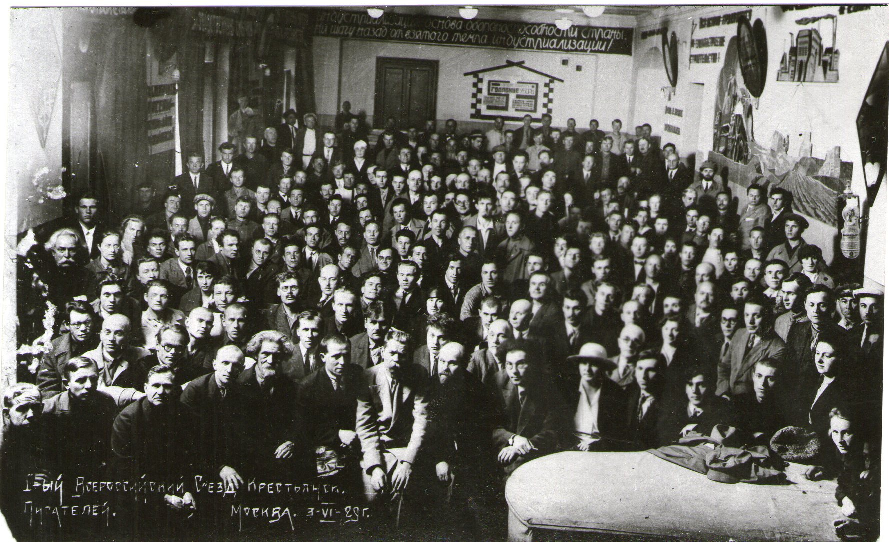
\includegraphics[width=0.9\textwidth]{syezd.pdf}
  \caption*{\centering1-й всероссийский съезд крестьянских писателей (Москва, 3 июня 1929 года)}
\end{figure}

\begin{figure}
  \centering
  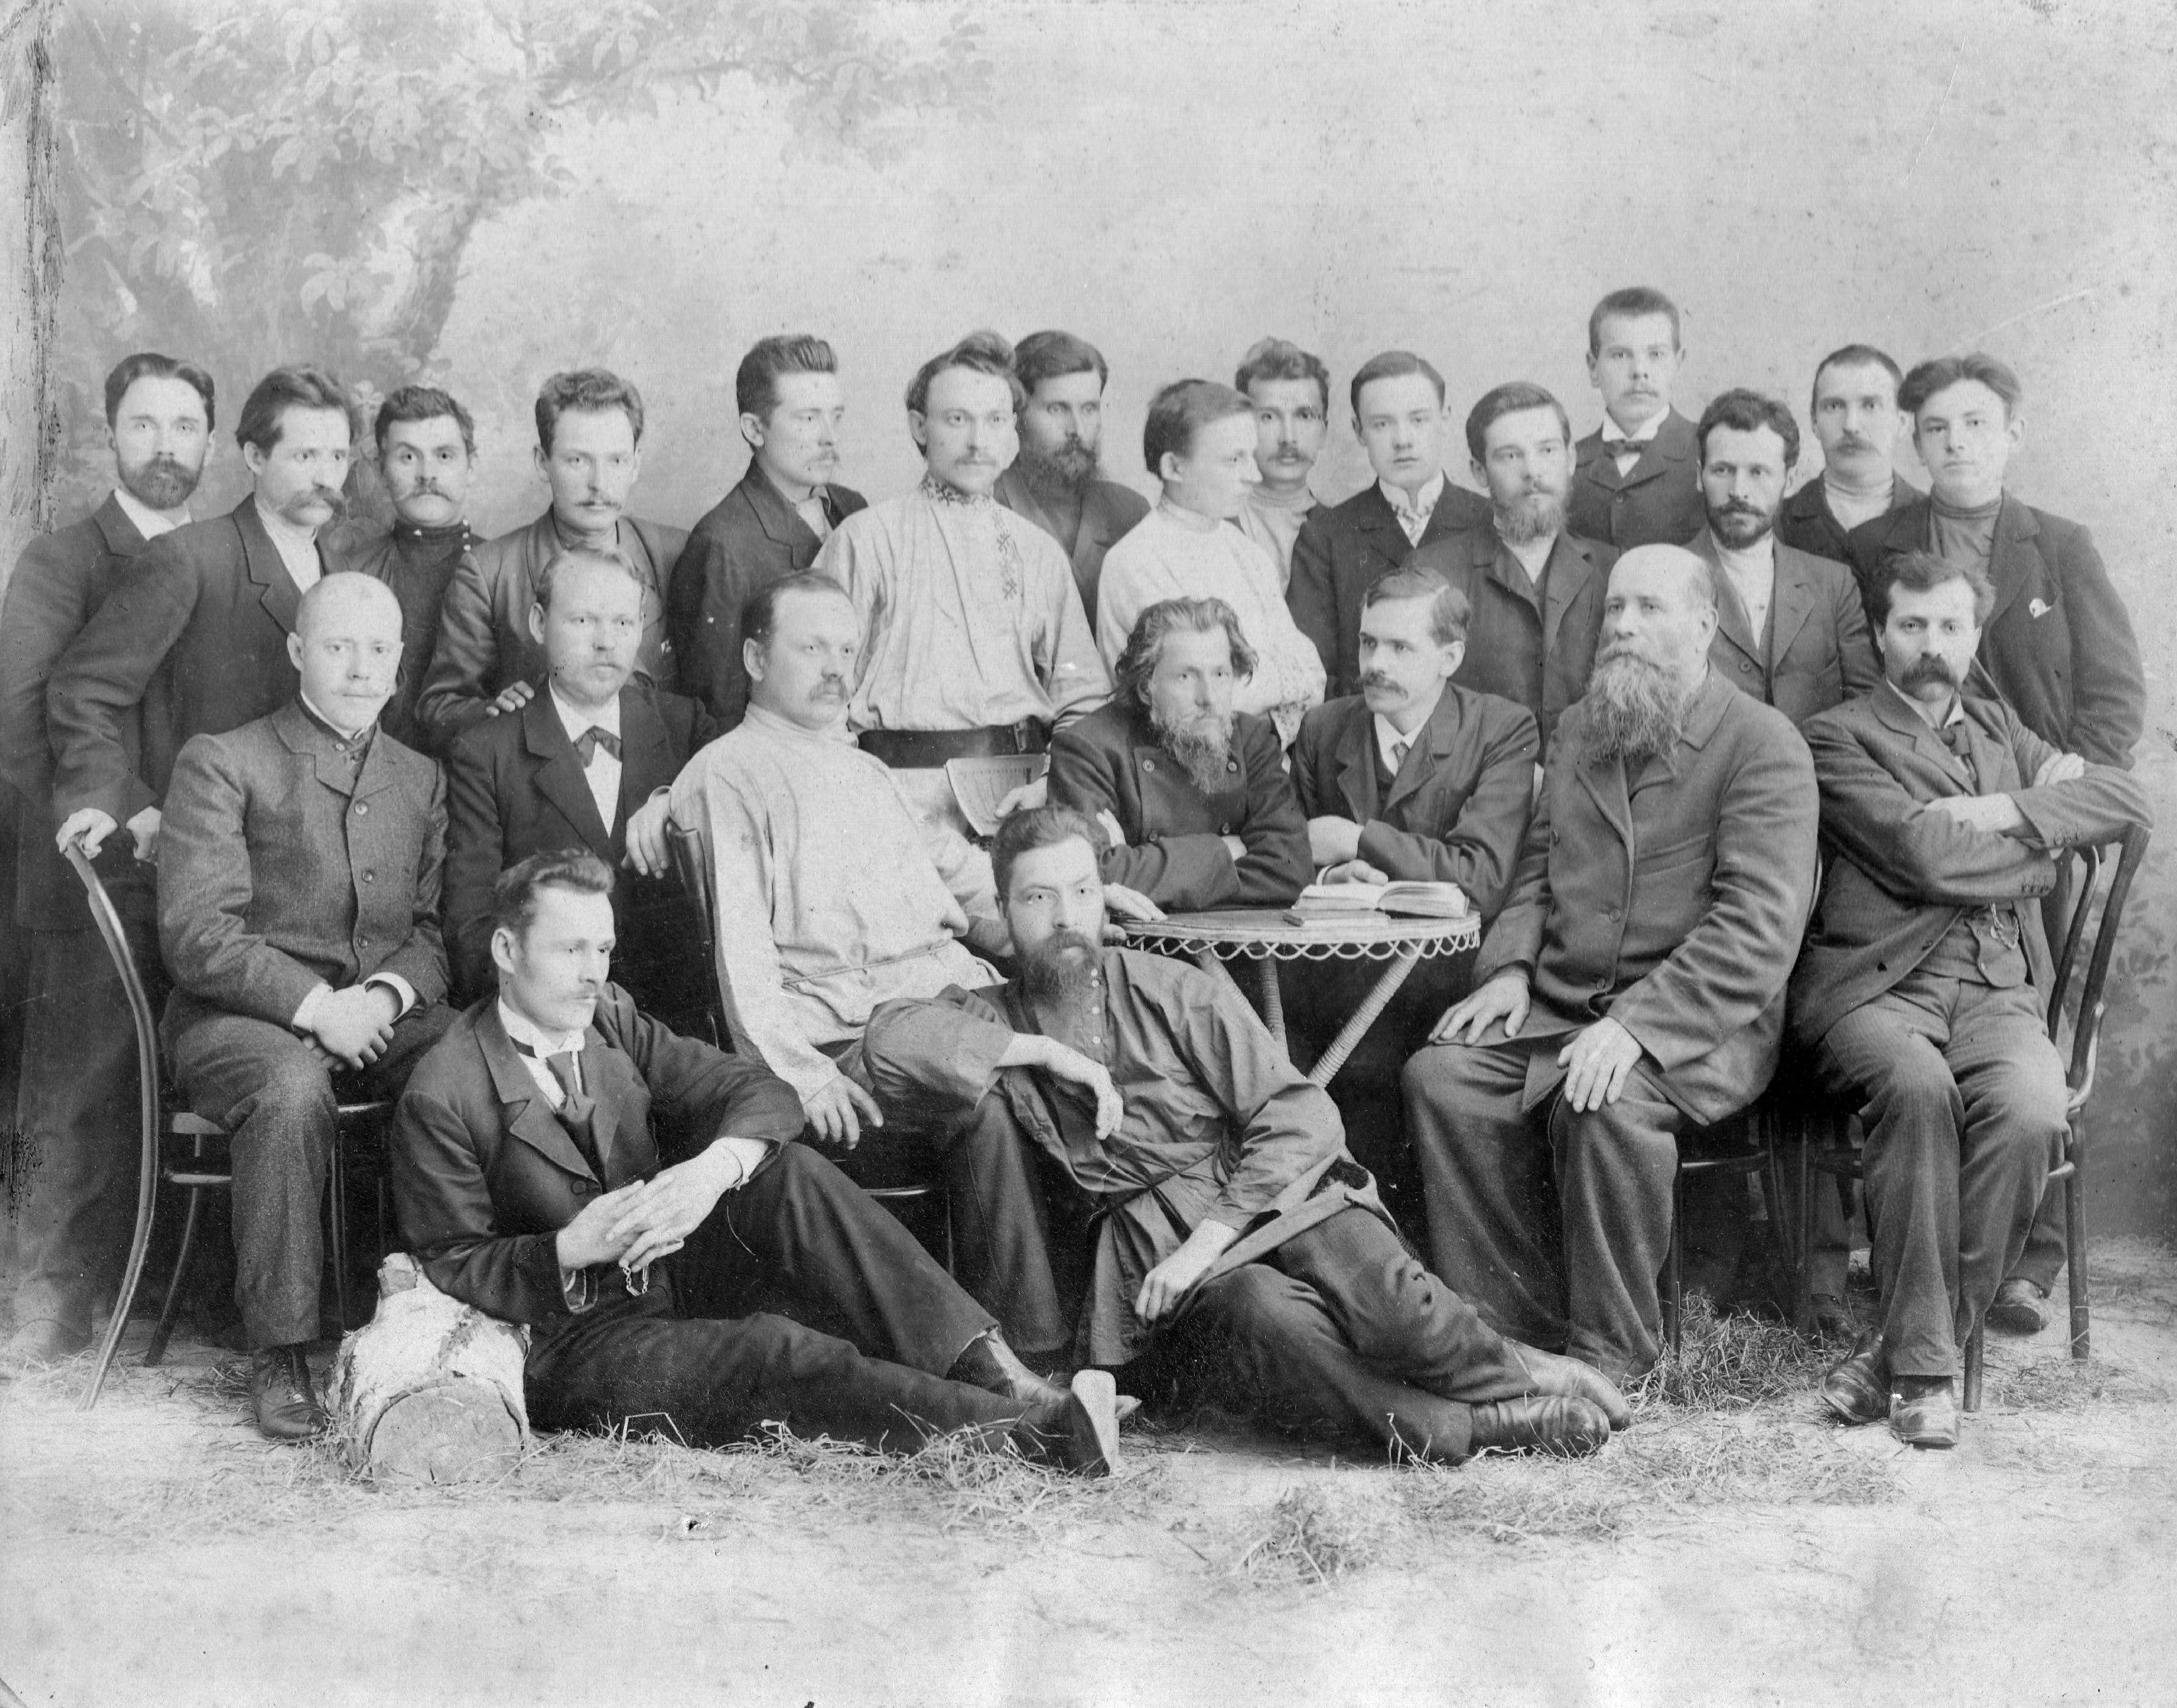
\includegraphics[width=0.9\textwidth]{pisateli.pdf}
  \caption*{Писатели и интеллигенция волоколамского уезда. Егор Кузьмичёв (4-й слева в последнем ряду), Федор Шкулев (2-й слева во втором ряду), Подъячев Семён (?) (3-ый справа во втором ряду), Спиридон Дрожжин (4-ий слева во втором ряду). Предположительно здесь есть Николай Михайлов, Сергей Ганьшин}
\end{figure}




% Оглавление

\renewcommand{\baselinestretch}{0.915}\normalsize
\tableofcontents
\renewcommand{\baselinestretch}{1.0}\normalsize



\end{document}
